\section{Generating Correlated Poisson Variables}\label{ch:generate_correlated_poisson}
In presenting the simulation procedure, it is necessary to discuss the method for generating correlated Poisson processes. The goal is to generate a multivariate random variable $\boldsymbol{X} = (X_1, X_2, \ldots, X_d)$ with mean $(\lambda_1, \lambda_2, \ldots, \lambda_{d})$ and $d$x$d$ correlation matrix $R$ where each $X_i$ has a marginal distribution that is the same as the distribution of a Poisson variable with mean $\lambda_i$. That is, $P(X_i = x_i) = f_i(x_i)$, where $f_i$ is the probability mass function of a Poisson variable with mean $\lambda_i$. \cite{A8} describes a procedure for generating $\boldsymbol{X}$ using the copula approach. 

A copula is defined as any joint probability distribution function where each marginal distribution is uniformly distributed (\cite{B1}). That is, 

$$C(\boldsymbol{u}): [0,1]^d \to [0,1]$$ 

is a copula if $C(0, 0, \ldots, 0) = 0$ and $C(1, \ldots, 1, u_i, 1, \ldots, 1) = u_i$ and $u_i \in [0,1]$ for all $i$. The Gaussian copula as described in \cite{A8} is used, where

$$ C_R^{Gaussian}(u_1, u_2, \ldots, u_d) = \Phi_{R}(\Phi^{-1}(u_1), \Phi^{-1}(u_2), \ldots,  \Phi^{-1}(u_d))$$

where $\Phi$ is the cumulative distribution function for a standard random normal variable and $\Phi_{R}$ is the cumulative distribution function for a random multivariate normal vector with mean $0$, variance $1$, and correlation matrix $R$. $u$ can be generated by first generating a multivariate normal random variable $Y = (Y_1,Y_2, \ldots, Y_d)$ with correlation matrix $R$ and setting $(u_1, u_2, \ldots, u_d) = (\Phi(y_1), \Phi(y_2), \ldots,  \Phi(y_d))$. It can then be paired with a copula that has marginal Poisson distributions. Namely,

$$ C^{Poisson}(F_1(x_1), F_2(x_2), \ldots, F_d(x_d))$$ where $F_i$ is the discrete cumulative distribution function for a Poisson random variable with rate $\lambda_i$. $x$ can then be set to

$$(x_1, x_2, \ldots, x_d) = (F^{-1}_1(u_1), F^{-1}_2(u_2), \ldots, F^{-1}_d(u_d))$$

To implement $F^{-1}_i(u_i)$, the inverse transform method as described in \cite{B1} is used:
\newline

\begin{algorithm}[H]
\SetAlgoLined
\caption{Inverse Transform Method for Generating a Poisson Rate Variable With Mean $\lambda$ and quantile $u$}
 $i \leftarrow 0$\;
 $p \leftarrow e^{-\lambda}$\;
 $F \leftarrow p$\;
 \While{$u \geq F$}{
  $p \leftarrow \lambda p / (i + 1)$ \;
  $F \leftarrow F + p$ \;
  $i \leftarrow i + 1$ \;
 }
 return $i$ \;
\end{algorithm}

Each $x_i$ will have a marginal Poisson distribution with rate $\lambda_i$ and $x$ will approximately have correlation matrix $\sigma$. Table \ref{tab:experimental_correlation} shows the accuracy of this method for different desired correlations. For each desired correlation 10000 pairs of random variables $(x_1,x_2)$ are generated that have means $1$ and joint Poisson distribution (see Listing \ref{correlated-poisson}). For each correlation level $x_1$ and $x_2$ have the correct means that are very near 1. For positive correlations, the actual correlation is slightly below the desired correlation (less than 0.1 difference at each desired correlation). For negative correlations, the actual correlation is slightly above the desired correlation for smaller magnitudes and deviates significantly at higher magnitudes. In practice, our correlation matrix $\sigma$ contains values that range from small negative to large positive correlations (see Tables \ref{tab:pos_pos_corr_tab}, \ref{tab:pos_neg_corr_tab}, and \ref{tab:neg_neg_corr_tab}), so this method would generate Poisson arrivals that follow $\sigma$ relatively closely. It may be possible to generate arrivals that more accurately reflect the given correlations, but this method provides acceptable performance given our needs.

\begin{table}
\label{tab:experimental_correlation}
\centering
\caption{Actual vs. Desired Correlation Using Gaussian Copula, $n=10000$}
\begin{tabular}{l|l|l|l}
\hline \hline
\textbf{Desired Correlation} & $\bar{x_1}$ & $\bar{x_2}$ & \textbf{Actual Correlation}  \\ 
\hline
-1                  & 0.995                           & 1.009                           & -0.735              \\
-0.9                & 0.997                           & 0.997                           & -0.682              \\
-0.8                & 1.01                            & 0.985                           & -0.616              \\
-0.7                & 0.987                           & 1.003                           & -0.543              \\
-0.6                & 0.99                            & 1.014                           & -0.472              \\
-0.5                & 0.998                           & 1.002                           & -0.405              \\
-0.4                & 1.016                           & 0.988                           & -0.308              \\
-0.3                & 1.003                           & 1.005                           & -0.236              \\
-0.2                & 1.001                           & 1.007                           & -0.163              \\
-0.1                & 0.998                           & 1.018                           & -0.086              \\
0                   & 1.014                           & 0.986                           & 0.016               \\
0.1                 & 0.976                           & 0.992                           & 0.062               \\
0.2                 & 0.994                           & 0.986                           & 0.162               \\
0.3                 & 0.995                           & 1.002                           & 0.246               \\
0.4                 & 1.006                           & 1.004                           & 0.371               \\
0.5                 & 1                               & 0.997                           & 0.433               \\
0.6                 & 0.987                           & 1.001                           & 0.522               \\
0.7                 & 1.007                           & 1.007                           & 0.616               \\
0.8                 & 0.993                           & 0.986                           & 0.727               \\
0.9                 & 1.01                            & 1.008                           & 0.829               \\
1                   & 0.997                           & 0.997                           & 1                  
\end{tabular}
\end{table}

\section{Backwards Simulation} \label{ch:backwards_simulation}

Using the methods in Section \ref{ch:generate_correlated_poisson}, the numbers of positive and negative events in a time period of length $t$ can be generated with means equal to $\lambda^{\pm}_k \cdot t$ and correlation matrix $\sigma$. Given the numbers of arrivals, a method called backwards simulation can be used to simulate the times of events (\cite{A7}). 

Backwards simulation uses the fact that conditioned on the number of arrivals in a Poisson process in a time period $t$ being equal to $n$, these arrivals are distributed uniformly across $[0,t)$. Using this method, arrivals over a large time period $T$ (i.e. $T = 10t$) can be generated by simulating arrivals in smaller chunks of size $t$. An algorithm is presented below for simulating arrivals over a time period $[s,s+t)$, with the arrivals following a $4K$ multivariate Poisson process. The event sizes are distributed exponentially with means $\mu^{\pm}_k$ as described in Section \ref{ch:poisson}. It returns a list of events $E$ whose entries $(k,y,\tau)$ are the event position, size, and time respectively:
\newline

\begin{algorithm}[H]
\label{alg:backwards_simulation}
\SetAlgoLined
\caption{Backwards Simulation Method For Generating Correlated Poisson Arrivals During Time Period $[s, s+t)$}
 $E = []$;

 Generate Poisson variables $(n^{\pm}_{-K}, \ldots, n^{\pm}_{-1}, n^{\pm}_1, \ldots, n^{\pm}_K)$ with means $(\lambda^{\pm}_{-K}, \ldots, \lambda^{\pm}_{-1}, \lambda^{\pm}_1, \ldots, \lambda^{\pm}_K)$ and correlation matrix $\sigma$ (see Section \ref{ch:generate_correlated_poisson}) \;
 
 \For{$k = -K, \ldots, -1, 1, \ldots, K$} {
    \For{$i = 1, \ldots, n^+_k$} {
        Generate $\tau$ $\sim$ Uniform($s$, $s+t$) \;
        Generate $y$ $\sim$ Exponential($\mu^+_k$) \;
        Append $(k,y,\tau)$ to $E$ \;
    }
    \For{$i = 1, \ldots, n^-_k$} {
        Generate $\tau$ $\sim$ Uniform($s$, $s+t$) \;
        Generate $y$ $\sim$ Exponential($\mu^-_k$) \;
        Append $(k,-y,\tau)$ to $E$ \;
    }
 }
 
 Return $E$ \;
 
\end{algorithm}

$$ $$

Sample arrivals using the parameters estimated in Chapter \ref{ch:experiment} are shown in Figures \ref{fig:bid_events_graphs} and \ref{fig:ask_events_graphs}. Positive events are shown in blue while negative events are shown in orange.

\begin{figure}
\centering
\caption{Bid Arrivals over $T$ = 600 seconds}
\begin{tabular}{cc}
\hline
\subf{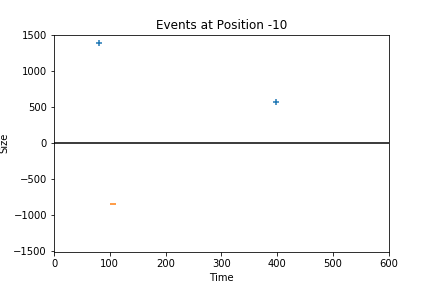
\includegraphics[width=60mm]{Figures/Events/events-10.png}}
{}
&
\subf{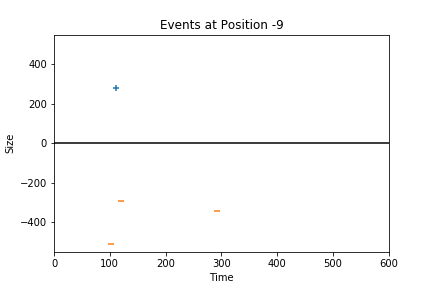
\includegraphics[width=60mm]{Figures/Events/events-9.png}}
{}
\\
\subf{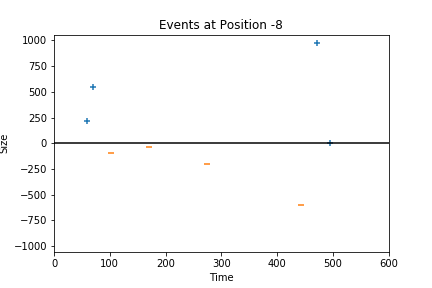
\includegraphics[width=60mm]{Figures/Events/events-8.png}}
{}
&
\subf{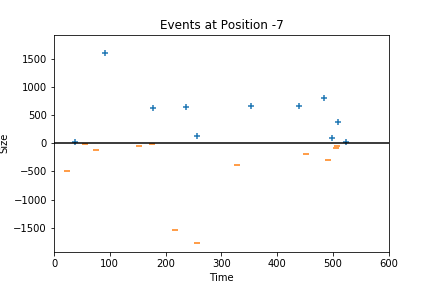
\includegraphics[width=60mm]{Figures/Events/events-7.png}}
{}
\\
\subf{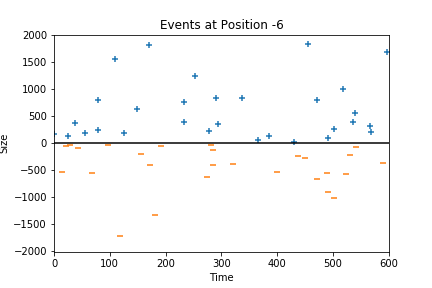
\includegraphics[width=60mm]{Figures/Events/events-6.png}}
{}
&
\subf{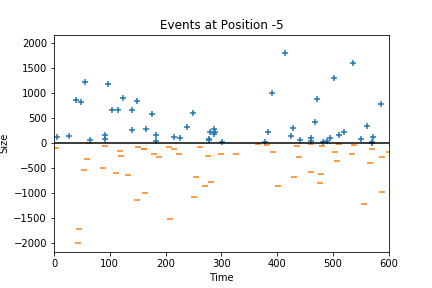
\includegraphics[width=60mm]{Figures/Events/events-5.png}}
{}
\\
\subf{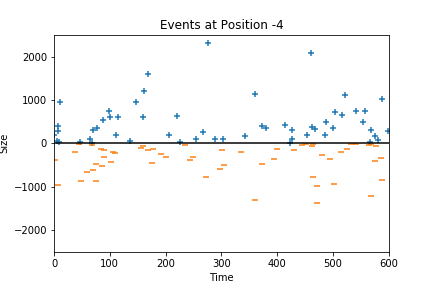
\includegraphics[width=60mm]{Figures/Events/events-4.png}}
{}
&
\subf{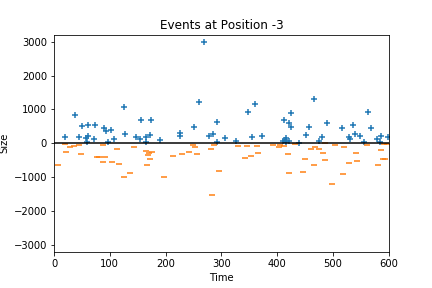
\includegraphics[width=60mm]{Figures/Events/events-3.png}}
{}
\\
\subf{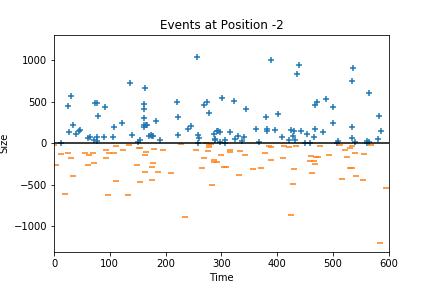
\includegraphics[width=60mm]{Figures/Events/events-2.png}}
{}
&
\subf{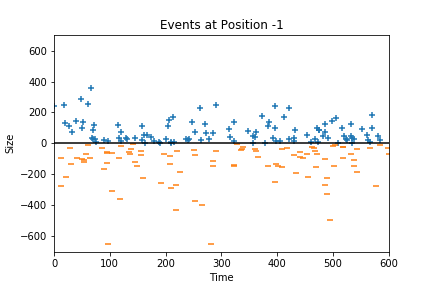
\includegraphics[width=60mm]{Figures/Events/events-1.png}}
{}
\\
\hline
\end{tabular}
\label{fig:bid_events_graphs}
\end{figure}

\begin{figure}
\centering
\caption{Ask Arrivals over $T$ = 600 seconds}
\begin{tabular}{cc}
\hline
\subf{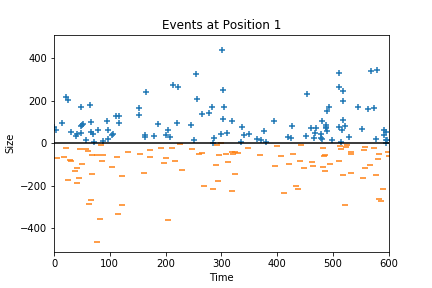
\includegraphics[width=60mm]{Figures/Events/events1.png}}
{}
&
\subf{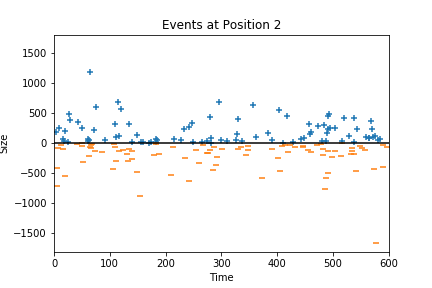
\includegraphics[width=60mm]{Figures/Events/events2.png}}
{}
\\
\subf{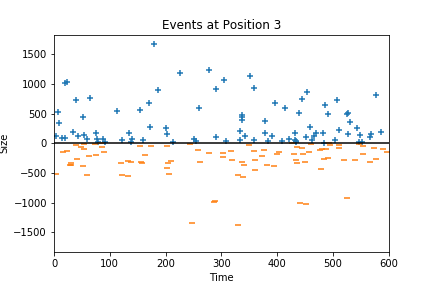
\includegraphics[width=60mm]{Figures/Events/events3.png}}
{}
&
\subf{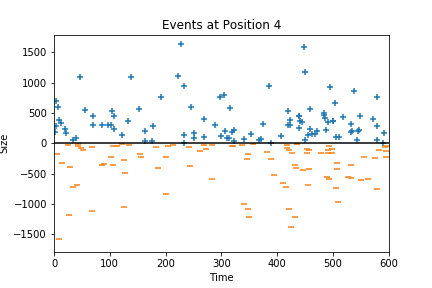
\includegraphics[width=60mm]{Figures/Events/events4.png}}
{}
\\
\subf{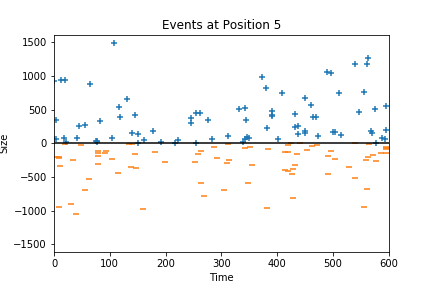
\includegraphics[width=60mm]{Figures/Events/events5.png}}
{}
&
\subf{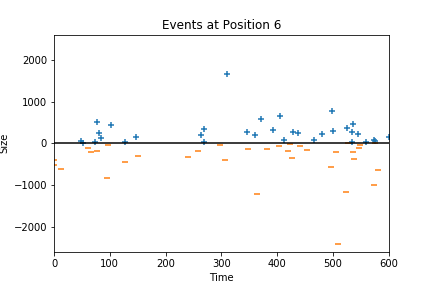
\includegraphics[width=60mm]{Figures/Events/events6.png}}
{}
\\
\subf{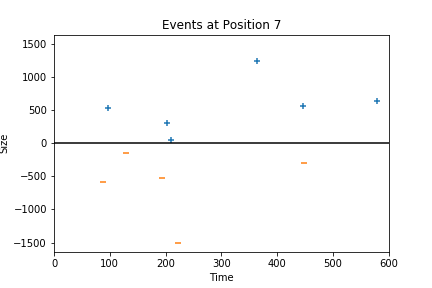
\includegraphics[width=60mm]{Figures/Events/events7.png}}
{}
&
\subf{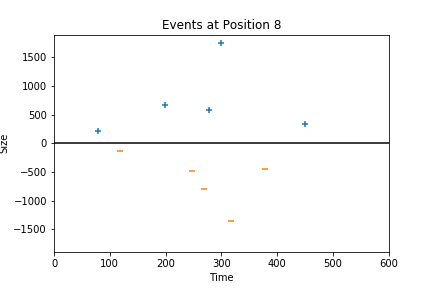
\includegraphics[width=60mm]{Figures/Events/events8.png}}
{}
\\
\subf{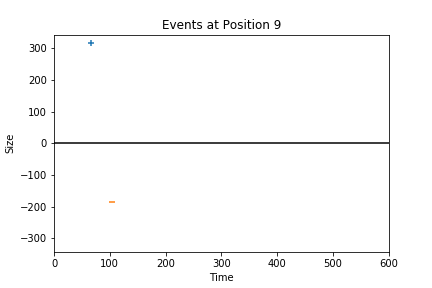
\includegraphics[width=60mm]{Figures/Events/events9.png}}
{}
&
\subf{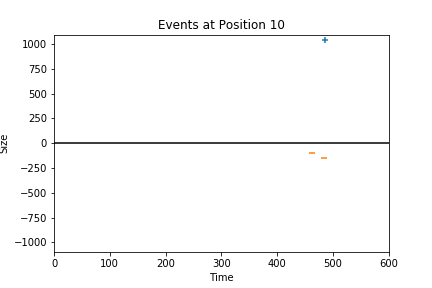
\includegraphics[width=60mm]{Figures/Events/events10.png}}
{}
\\
\hline
\end{tabular}
\label{fig:ask_events_graphs}
\end{figure}

\section{Simulation Algorithm} \label{ch:simulation_algorithm}

The actions of the agent can now be incorporated into the simulation. I assume that the agent needs to buy at least $V$ units in a time period $T$ and submits orders of the form $(a,\tau)$ which indicates a market buy order for amount $a$ at time $\tau$. At the end of the time period, if $A$ units have not been bought, then the trader makes a market order for the remainder of the inventory. External events on the order book are generated using the algorithm described in section \ref{ch:backwards_simulation}, and the reference price is updated as described in \ref{ch:queue_model}. The agent's market buys are executed at the best available price, and the simulation returns a list of executed trades of the form $(p,a,\tau)$, which contains the price, amount, and time of the trade.

See Listing \ref{code:simulation} for the code written to perform this simulation.

\begin{algorithm}[H]
\SetAlgoLined
\caption{Simulation of Order Book: Setup and Input}
Let $p_{ref}$ be the starting reference price ;

Let $L$ be the initial LOB at time $0$. Let $L_p$ be the volume at price $p$ ;

Let $v$ be the amount of inventory filled ;

Let $O$ be the trades executed ;

Let $\Theta$ be the list of orders of the form $(a,\tau)$ If $\sum{a} < V$, append $(V - \sum{a}, T)$ to $\Theta$;

Generate $E$ using Algorithm \ref{alg:backwards_simulation} $E$ contains events of form $(k,c,\tau)$ where $k$ is the position in relation to the reference price, $c$ is the change, and $\tau$ is the time ;

Sort $\Theta$ and $E$ by $\tau$ ;
\end{algorithm}

\begin{algorithm}[H]
\SetAlgoLined
\caption{Simulation of Order Book: Tracking Market Orders}
Proceed through $\Theta$ and $E$ in time order. 

\While{$\tau <= T$ and $v < V$} {
    \If {\text{event of form} $(k,c,\tau)$} {
        convert $k$ to price $p$ ;
        \If {$c > 0$} {
            $L_p \leftarrow L_p + c$ ;
        }
        \Else {
            \If {\text{Best bid or best ask}} {
                Let $\eta = c$;
                \While {$\eta < 0$} {
                    $L_p \leftarrow max(0,L_p + \eta)$ ;
                    
                    $\eta \leftarrow \eta + max(L_p, -\eta)$ ;
                    
                    Set $p$ to be the next best price ;
                }
            }
            \Else {
                $L_p \leftarrow max(0,L_p + c)$ ;
            }
        }
    }
    \If {\text{order of form} $(a,\tau)$} {
        Let $p$ be the best ask ;
        Let $\eta = c$ ;
        \While {$\eta < 0$} {
            $L_p \leftarrow max(0,L_p + \eta)$ ;
            
            Append $(p,max(L_p, -\eta), \tau)$ to $O$ ;

            $\eta \leftarrow \eta + max(L_p, -\eta)$ ;
            
            $p \leftarrow p + 1$ ;
        }
    }
}

Return $O$ ;
\end{algorithm}







